\begin{figure}[htb]
\begin{subfigure}[t]{0.4\textwidth}
    \centering
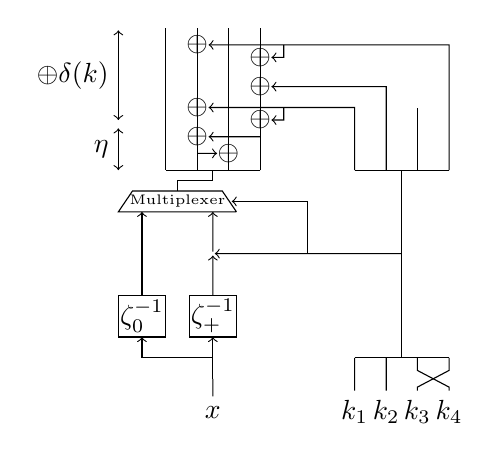
\begin{tikzpicture}[xscale=-0.6, yscale=-0.53]
        % Input bits
        \draw
        (-3.00, 2.80) node(k3){$k_{4}$} 
        (-2.33, 2.80) node(k2){$k_{3}$} 
        (-1.67, 2.80) node(k1){$k_{2}$} 
        (-1.00, 2.80) node(k0){$k_{1}$} ;
%        \draw (-3.00, 1.50) -- (k3);
%        \draw (-2.33, 1.50) -- (k2);
%        \draw (-1.00, 1.50) -- (-1.00, 1.80) -- (-1.67, 2.20) -- (k1);
%        \draw (-1.67, 1.50) -- (-1.67, 1.80) -- (-1.00, 2.20) -- (k0);
        \draw (-3.00, 1.50) -- (-3.00, 1.8) -- (-2.33, 2.2) -- (k2);
        \draw (-2.33, 1.50) -- (-2.33, 1.8) -- (-3.00, 2.2) -- (k3);
        \draw (-1.00, 1.50) -- (-1.00, 2.20) -- (k0);
        \draw (-1.67, 1.50) -- (-1.67, 2.20) -- (k1);

        \draw (-3.00, 1.50) -- (-1.00, 1.50) ;

        % Mini S-Boxes
        \draw (+1.5, +0.0) rectangle (+2.5, +1.0) node[pos=0.5] {$\zeta_{+}^{-1}$} ;
        \draw (+3.0, +0.0) rectangle (+4.0, +1.0) node[pos=0.5] {$\zeta_{0}^{-1}$} ;
        \draw (+2.0, -1.0) node[inner sep=0] (mult) {$\fmult$};
        % 4-bits wires
        % left
        \draw     (-2.0, +1.5) -- (-2.0, -3.0) ;
        \draw[->] (-2.0, -1.0) -- (mult) ;
        % right
		\draw (+2, 2.8) node(x){$x$};
		\draw (x) -- (2, 2);
        \draw     (+2.00, +2.00) -- (+2.0, +1.5) -- (+3.5, +1.5) ;
        \draw[->] (+2.0, +1.5) -- (+2.0, +1.0) ;
        \draw[->] (+3.5, +1.5) -- (+3.5, +1.0) ;
        \draw[->] (+2.0, +0.0) -- (mult);
        \draw[->] (mult) -- (+2.0, -2.0);
        \draw[->] (+3.5, +0.0) -- (+3.5, -2.0);
        % multiplexer
        \draw (+1.5, -2.00) -- (+4.0, -2.00) -- (+3.70, -2.5) -- (+1.8, -2.5) -- (+1.5, -2.00) ;
        \draw[->] (+0.00, -1.00) -- (+0.00, -2.25) -- (+1.6, -2.25);
        \draw (+2.75, -2.5) -- (+2.75, -2.75) -- (+2.0, -2.75) -- (+2.0, -3.00);
        \draw (+2.75, -2.25) node{\tiny Multiplexer};
        % ciphertext bits
        \draw
        (+1.00, -3.00) -- (+3.00, -3.00)
        (+1.00, -3.00) -- (+1.00, -6.40)
        (+1.67, -3.00) -- (+1.67, -6.40)
        (+2.33, -3.00) -- (+2.33, -6.40)
        (+3.00, -3.00) -- (+3.00, -6.40) ;
        % u_f
        \draw
        (+2.33, -3.40) coordinate(uf1_source) (+1.67, -3.40) node[inner sep=0](uf1_target){$\oplus$}
        (+1.00, -3.80) coordinate(uf2_source) (+2.33, -3.80) node[inner sep=0](uf2_target){$\oplus$};
        \draw[->] (uf1_source) -- (uf1_target);
        \draw[->] (uf2_source) -- (uf2_target);
        % end key bits

		\draw (2.33, -4.5) node[inner sep=0](xor01) {$\oplus$};
		\draw (2.33, -6) node[inner sep=0](xor21) {$\oplus$};
		\draw (1.00, -5) node[inner sep=0](xor13) {$\oplus$};
		\draw (1.00, -4.2) node[inner sep=0](xor03) {$\oplus$};
		\draw (1.00, -5.7) node[inner sep=0](xor23) {$\oplus$};

        \draw        (-3.00, -3.00) -- (-1.00, -3.00);

        \draw[->]        (-3.00, -3.00) -- (-3.00, -6) -- (xor21);
        \draw[->]                     (0.5, -6) -- (0.5, -5.7) -- (xor23);
        \draw        (-2.33, -3.00) -- (-2.33, -4.5);
        \draw[->]        (-1.67, -3.00) -- (-1.67, -5) -- (xor13);
        \draw[->]        (-1.00, -3.00) -- (-1.00, -4.5) -- (xor01);
        \draw[->]                     (0.5, -4.5) -- (0.5, -4.2) -- (xor03);



        % u_out

%        \draw        (-1.00, -4.50) coordinate(out1_source) (+3.00, -4.50) node[inner sep=0](out1_target){$\oplus$};
%        \draw        (+1.67, -4.75) node[inner sep=0](out2_target){$\oplus$};
%        \draw        (-2.33, -5.25) coordinate(out3_source) (+3.00, -5.25) node[inner sep=0](out3_target){$\oplus$};
%        \draw        (-3.00, -5.75) coordinate(out4_source) (+3.00, -5.75) node[inner sep=0](out4_target){$\oplus$};
%        \draw        (+1.67, -6.00) node[inner sep=0](out5_target){$\oplus$};
        
%        \draw[->] (out1_source) -- (out1_target);
%        \draw[->] (+1.20, -4.50) -- (+1.20, -4.75) -- (out2_target);
%        \draw[->] (out3_source) -- (out3_target);
%        \draw[->] (out4_source) -- (out4_target);
%        \draw[->] (+1.20, -5.75) -- (+1.20, -6.00) -- (out5_target);
        % Explanations
        % \draw[<->] (+4.5, -1.9) -- node[right]{\tiny Multi- plexer} (+4.5, -2.6);
        \draw[<->] (+4, -3.0) -- node[left]{$\eta$} (+4, -4.0);
        \draw[<->] (+4, -4.2) -- node[left]{$\oplus \delta(k)$} (+4, -6.35);
      \end{tikzpicture}
\end{subfigure}
    %\FigDef{final-t}{Final decomposition of $T^{-1}_k(x)$.}}
\begin{subfigure}[t]{0.58\textwidth}
\vspace{-5cm} % hack..
    \centering
      \renewcommand\arraystretch{1.3}
      \setlength{\tabcolsep}{2pt}
      \footnotesize
      \centering
      \begin{tabular}{l|rrrrrrrrrrrrrrrr}
 ~&~ $\hex{0}$ & $\hex{1}$ & $\hex{2}$ & $\hex{3}$ & $\hex{4}$ & $\hex{5}$ & $\hex{6}$ & $\hex{7}$ & $\hex{8}$ & $\hex{9}$ & $\hex{a}$ & $\hex{b}$ & $\hex{c}$ & $\hex{d}$ & $\hex{e}$ & $\hex{f}$\\
        \hline
$\delta$ ~&~ $\hex{0}$ & $\hex{0}$ & $\hex{5}$ & $\hex{5}$ & $\hex{1}$ & $\hex{1}$ & $\hex{4}$ & $\hex{4}$ & $\hex{5}$ & $\hex{5}$ & $\hex{0}$ & $\hex{0}$ & $\hex{4}$ & $\hex{4}$ & $\hex{1}$ & $\hex{1}$\\
$\eta$ ~&~ $\hex{0}$ & $\hex{5}$ & $\hex{2}$ & $\hex{7}$ & $\hex{6}$ & $\hex{3}$ & $\hex{4}$ & $\hex{1}$ & $\hex{8}$ & $\hex{d}$ & $\hex{a}$ & $\hex{f}$ & $\hex{e}$ & $\hex{b}$ & $\hex{c}$ & $\hex{9}$\\
$\swaplsb$ ~&~ $\hex{0}$ & $\hex{2}$ & $\hex{1}$ & $\hex{3}$ & $\hex{4}$ & $\hex{6}$ & $\hex{5}$ & $\hex{7}$ & $\hex{8}$ & $\hex{a}$ & $\hex{9}$ & $\hex{b}$ & $\hex{c}$ & $\hex{e}$ & $\hex{d}$ & $\hex{f}$\\
$\zeta_0$ ~&~ $\hex{2}$ & $\hex{5}$ & $\hex{3}$ & $\hex{b}$ & $\hex{6}$ & $\hex{9}$ & $\hex{e}$ & $\hex{a}$ & $\hex{0}$ & $\hex{4}$ & $\hex{f}$ & $\hex{1}$ & $\hex{8}$ & $\hex{d}$ & $\hex{c}$ & $\hex{7}$\\
$\zeta_+$ ~&~ $\hex{7}$ & $\hex{6}$ & $\hex{c}$ & $\hex{9}$ & $\hex{0}$ & $\hex{f}$ & $\hex{8}$ & $\hex{1}$ & $\hex{4}$ & $\hex{5}$ & $\hex{b}$ & $\hex{e}$ & $\hex{d}$ & $\hex{2}$ & $\hex{3}$ & $\hex{a}$\\
$\inv$ ~&~ $\hex{0}$ & $\hex{1}$ & $\hex{c}$ & $\hex{8}$ & $\hex{6}$ & $\hex{f}$ & $\hex{4}$ & $\hex{e}$ & $\hex{3}$ & $\hex{d}$ & $\hex{b}$ & $\hex{a}$ & $\hex{2}$ & $\hex{9}$ & $\hex{7}$ & $\hex{5}$\\

      \end{tabular}
\end{subfigure}
    %} {\TabDef{t-books}{Functions used in the decomposition of $T$.}} 
  %\end{floatrow}
  \FigDef{final-t}{The decomposition of $T^{-1}_k(x)$.}
\end{figure}